%\documentclass{beamer}
\documentclass[xcolor=pdftex,dvipsnames,table]{beamer}
\usepackage{verbatim}
\usepackage{amsmath}

\usetheme{Luebeck}
\usecolortheme[named=RawSienna]{structure}
\setbeamerfont{frametitle}{family=\rmfamily,shape=\itshape}
%\setbeamertemplate{frametitle}[default][center]
\defbeamertemplate*{title page}{customized}[1][]
{
  \vspace{1.9cm}

% Content
  \begin{minipage}{10cm}

  % Title and subtitle
  \begin{beamercolorbox}[center,#1]{title}
    \vskip0.04em%
    \usebeamerfont{title}\inserttitle\par%
    \ifx\insertsubtitle\@empty%
    \else%
      \vskip0.3em%
      {\usebeamerfont*{subtitle}\usebeamercolor*[fg]{subtitle}\insertsubtitle\par}%
    \fi%
    \vskip0.3em%
  \end{beamercolorbox}%

  \vskip1em\par

  % Display author(s)
  \begin{beamercolorbox}[center,#1]{author}
    \usebeamerfont{author}\insertauthor{}
  \end{beamercolorbox}

  \vskip1em\par

  % Institute
  \begin{beamercolorbox}[center,#1]{institute}
    \usebeamerfont{institute}\insertinstitute{}
  \end{beamercolorbox}

  \vskip1em%

  % Date
  \begin{beamercolorbox}[center,#1]{date}
    \usebeamerfont{date}\insertdate
  \end{beamercolorbox}\vskip0.5em

  \end{minipage}
  \hspace{0.6cm}
  \vfill

  \begin{flushleft}
  {\usebeamercolor[fg]{titlegraphic}\inserttitlegraphic\par}
  \end{flushleft}
  \hfill

%  \usebeamerfont{title}\inserttitle\par
%  \usebeamerfont{subtitle}\usebeamercolor[fg]{subtitle}\insertsubtitle\par
%  \bigskip
%  \usebeamerfont{author}\insertauthor\par
%  \usebeamerfont{institute}\insertinstitute\par
%  \usebeamerfont{date}\insertdate\par
%  \usebeamercolor[fg]{titlegraphic}\inserttitlegraphic
}

\title{The Rubik's Cube and Group Theory}
\subtitle{"In mathematics you don’t understand things. You just get used to them." - J. von Neumann}
\author{David Buchmann}
\institute{Cisco Systems}

\date{\today}

\begin{document}

\maketitle

\section{Rubik's Cube Background}
\begin{frame}
  \frametitle{Kubik Rubik}
  \begin{columns}[cc]
    \column{2.5in}
    \begin{itemize}
    \item Erno Rubik (a Hungarian professor of Interior Design) created the Rubik's cube in 1974.
    \item 100,000,000 cubes have been sold worldwide.
    \item There are 26 visible cubies on the 3 by 3 Rubik's cube (8 corner cubies, 12 edge cubies, and 6 center cubies)
    \item God's number: Every Rubik's cube can be solved in 20 or less moves.
  \end{itemize}
    \column{0.5in}
    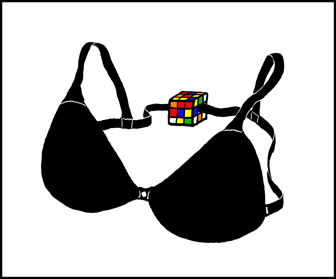
\includegraphics[scale=0.33]{rubik_frustration.png}
  \end{columns}
\end{frame}

\section{Group Theory}
\begin{frame}
  A group is a mathematical construct consisting of a set and an operation satisfying the following axioms:
  \begin{itemize}
    \item Associativity - operation must satisfy $(a + b) + c = a + (b + c)$
    \item Closure - applying the operation on any combination of elements in the set must yield another element inside the set.
    \item Inverse element - Every element in the set must have an inverse element
    \item Identity element - An element which is it's own inverse
  \end{itemize}
\end{frame}

\begin{frame}
  Example: The hours on a 12-hour clock forms a group under addition (and is denoted $ \mathbb{Z} / 12\mathbb{Z}$ or $\mathbb{Z}_{12}$ for short)
  \begin{itemize}
    \item 0 is the identity element
    \item Set {0,1,2,3,4,5,6,7,8,9,10,11}
    \item Operation is + modulo 12
  \end{itemize}
\end{frame}

\begin{frame}
  \frametitle{The Rubik's Group}
  \begin{itemize}
    \item 6 different colors
    \item The group representing the Rubik's cube ($ \mathbf{R} $) is a group where the elements are all possible permutations of the Rubik's cube, and the operation is concatenation of these permutations.
  \end{itemize}
\end{frame}

\section{The Rubik's Group}
\begin{frame}
  Any one permutation of the cube if applied enough times (order of the subgroup) will return you to your original position
  \begin{itemize}
    \item 
  \end{itemize}
\end{frame}

\begin{frame}
  \begin{itemize}
    \item
  \end{itemize}
\end{frame}

\end{document}
